%%This is a very basic article template.
%%There is just one section and two subsections.
\documentclass{article}

\usepackage{amsmath}
\usepackage{caption}
\usepackage{placeins}
\usepackage{graphicx}
\usepackage{subcaption}
\usepackage{tikz}
%\usepackage[active,tightpage]{preview}
\usepackage{natbib}
\bibpunct{(}{)}{,}{a}{}{;} 
\usepackage{url}
\usepackage{nth}
\usepackage{authblk}
% for the d in integrals
\newcommand{\dd}{\; \mathrm{d}}
\newcommand{\tc}{\quad\quad\text{,}}
\newcommand{\tp}{\quad\quad\text{.}}
\defcitealias{HMD}{HMD}
\defcitealias{HFD}{HFD}

\begin{document}


\title{Life lost, lifesaving, and causes of death.}

\author[1]{Tim Riffe\thanks{triffe@demog.berkeley.edu}}
\author[2]{A{\"i}da Sol\'{e} Aur\'{o}}
\affil[1]{Department of Demography, University of California, Berkeley}
\affil[2]{Universitat Pompeu Fabra}

\maketitle

% AS: I know that you said that this paper is not motivated by a substantive
 % research question, but I
%feel that there is a lack of the main research point. Why are you doing this
% investigation? Are you going to present various descriptive possible scenarios about mortality 
% impacts and potentials gains (in years of good/bad life). To address so, the
% abstract needs to explain, in a very synthetic way, what the reader will find in the full manuscript.
%
\begin{abstract}
We classify cause of death impacts on population stocks in five countries using
a counterfactual framework. The lives and potential years of life lost due to death are presented as a metric for describing the population impacts of death and for comparing causes of
death. Lost lives and years of life may be classified by the ages in which
deaths occurred, by the ages to which deaths would be postponed were they saved, by the
ages through which the lost years would have been lived, or by the distribution of
lost remaining lifespans. These temporal perspectives define the
potential impacts of death and causes of death on population size and structure,
and on the distribution of lifespans within populations. 
\end{abstract}

%There is a need for an introduction. A general framework to situate the reader,
% which concludes with a research question. We also need a paragraph to present
% the data you are willing to use, as well as years and countries. The
% introduction might structure a little bit what comes next: A) Temporal
% relationships, B) Extension to causes of death; C) Population comparisons.
%
\section*{Introduction}
A core task of demography is to account for and predict the population
pyramid and the forces that shape it. The pyramid represents population
size and age structure, and it is shaped by the flows of births,
deaths, and migrations\footnote{We are guilty of omitting migration from
the following exposition, although some of the methods presented here would
translate cleanly to emigration.}. Of these flows, births are usually regarded
as the primary driver of variation in the profile of the pyramid,\footnote{This
is true to the extent that wars, epidemics, and other mortality shocks effect
broad age ranges rather than abrupt age groups.} whereas the pattern of survival
exerts a gentler influence on the overall tapering and height of the pyramid.
Year to year variation in the number of deaths tends to deduct
smoothly from a wide range of ages, making mortality all but the most
severe mortality shocks illegible in the pyramid. This is perhaps why
relationships between mortality and age structure have been less charted than those between births and age structure.

Demographers most often quantify death in terms of age-specific rates via the
lifetable and its summary indices because these are considered purged of
accidental distortions from population age structure. Public health institutes and news media often also
report trends in absolute numbers of deaths from particular causes and the total potential years of life lost (YPLL) due to
these deaths.\footnote{\citet{gardner1990} review commonly used methods of
calculating YPLL. The Global Burden of Disease reports refer to YPLL as YLL.
As a news media example, in 2013 the Guardian ran a data blog entry
visualizing the years of life lost in the USA due to gun violence
\citep{rogers2013gun}. } In either of these treatments, mortality and deaths are
isolated from age structure. The notion of YPLL instead dovetails with
population size over time. 

In this paper our point of departure is to
treat deaths as age-structured population stocks through the notion of
potentially saveable life. Demography based on this step is a counterfactual exercise, in line with the formal treatment given in
\citet{vaupel1987repeated}.\footnote{\citet{vaupel2008lifesaving} follows in a
similar vein, but aims at the effects of lifesaving on period distortions.}
Saveable life and lifetime can be quantified flexibly with respect to demographic perspectives on age and lifespan. These perspectives refine and supplement YPLL when assessing the population impacts of causes of death, and we think that they would provide useful information for the targetting and planning
of public health interventions and the comparison of mortality burdens between
populations and subpopulations. The variety of visualizations presented here may
also enrich official periodic reporting on the absolute and relative population
impacts of causes of death.

We first formally define what is meant by age and lifespan
perspectives, illustrating on the example of all-cause
mortality before proposing an extention to causes of death. Concepts are
illustrated based on the population of the United States in 2010. We then
compare a selection of five contemporary national populations (United States, England \& Wales, Norway, Sweden and Canada) based on pre-release
data newly collected by the Human Mortality
Database~\citepalias{HMD}. We propose
a selection of strategies for visualizing and arranging results for purposes of
reporting or making comparisons. Finally we discuss the limits of these methods
and the utility of the information gained by them. All mortality data used in
the following comes from the HMD.

\section*{Temporal relationships}
% To begin, sume a closed population and ignore what determines the size of
% successive birth cohorts, $B(t)$, which we usually call the birth flow. If
% $B(t)$ is a given, then the only other factor that determines population size
% and age structure is the length of the lives of its members. For simplicity,
% assume that the age pattern to mortality is fixed (this isn't necessary, but
% it simplifies notation). The population of age $a$ in year $t$, $P(a,t)$, is a function of 
% the survival of the birth cohort born in year $t-a$. Since we're
% fixing mortality, survival from age 0 to $a$ is $l(a)$ for any given cohort,
% so $P(a,t) = B(t-a)l(a)$.

% AS: Temporal relationships: I really like this section, but I think it needs
% to be reordered. Starting from Figure 1, moving to Figure 2 which perfectly illustrates what you 
% can do (using different populations) to compute the average years of life
% left. But I suggest you to first describe the idea, what you have done at the
% bottom of page 2 and then say something like: "and this translates into the following 
% form"; therefore, you can add your formulas. Followed by Figure 3. Since I am
% writing this email as I am reading, I just realized that you need a paragraph in front to introduce
% what follows: a) lifetime; b) remaining years of life; c) potentially savable lives. I need to 
% think more about these figures, but the work is there.  

Population stock in a
 given year, $t$, can be structured by birth cohorts or age, the way we typically make 
 population pyramids. If an entire lifespan is denoted by the random variable
 $X$, then the remaining lifespan, $y$, of a still-alive person aged $a$, $y = X - a$.
\begin{figure}[h]
% Figure produced in R/LifeLine.R
\centering
	\caption{A lifeline, where chronological age (years lived) is indexed by $a$
	and thanatological age (years left) is indexed by $y$.}
	\label{fig:line}
	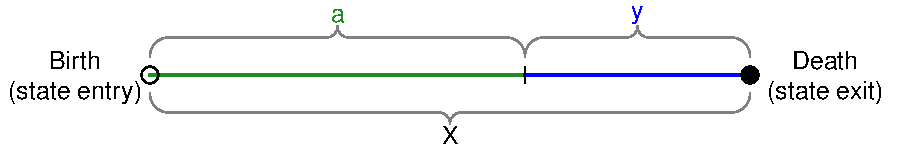
\includegraphics[scale=.8]{Figures/LifeLine.pdf}	
\end{figure}
Figure~\ref{fig:line} gives a schematic representation of this simple
relationship between age and the lifespan for a single person-life. The lived
part we call ``age'' and the yet-unlived part has no common name. Since age is a
placemarker on the lifeline, both $a$ and $y$ could be called ``age'', and we
can specify them as \textit{chronological} and \textit{thanatological} age,
respectively.\footnote{Thanatos was the Greek god of death, which marks the end of the lifeline to which $y$ relates. By this token, one could just call chronological age \textit{aphrodesian} age, but this would probably confuse things.}
The chronological and thanatological age perspectives are applicable to state
durations in general, but in this paper we focus on the full lifespan.

For a cohort, the distribution of $X$ is given by $f(X)$, which is equal to the
lifetable death distribution, $d(a)$, for $a = X$, when the lifetable is
specified with a radix equal to unity ($l(0)=1$).
The distribution of \textit{remaining} lifetime, $y$, for those having survived
to age $a$, $f(y|a)$ is given by:\footnote{This definition is identical to
that used in \citet{brouard1989mouvements}, \citet{vaupel2009life} or
\citet{rao2014generalization} in proving the equality of chronological and
thanatological age structure in stationary populations. Brouard apparently had
proven this earlier than 1989, since he cites the relationship in
\citet{brouard1986structure}. Equation \eqref{eq:fya} is easily modifiable to
account for mortality schedules that change over time.}
\begin{equation}
\label{eq:fya}
f(y|a) = \mu(a+y) \frac{l(a+y)}{l(a)} \tc
\end{equation}
where $\mu(a)$ is the force of mortality at exact age $a$, and $l(a)$ is
the value of the survival function at exact age $a$, proportional to the
probability of surviving from birth to age $a$. \eqref{eq:fya} can be expressed
in words as the probability of surviving $y$ years in the future given survival to current age $a$, and then dying at the exact age $a+y$.
Figure~\ref{fig:fya} shows selected cross-sections of the $f(y|a)$ surface calculated from the 2010 US male period
lifetable \citepalias{HMD}. The area under each chronological age-conditioned curve is equal to one.
As an individual grows older (here under a fixed mortality schedule), the
central mass of the curve approaches zero, moving one year down per year lived.
In these data, the shape of the center of the curve does not change much until
after chronological age 60, where conditional rescaling drives up death probabilities more and more. Upward
scaling continues beyond those ages shown here, with $y=0$ becoming the greatest
single value in all ages beyond the modal chronological age at death.

 \begin{figure}[h]
\centering
% Figure produced in R/fya.R
	\caption{US males, 2010, $f(y|a)$ for selected ages.*}
	\label{fig:fya}
	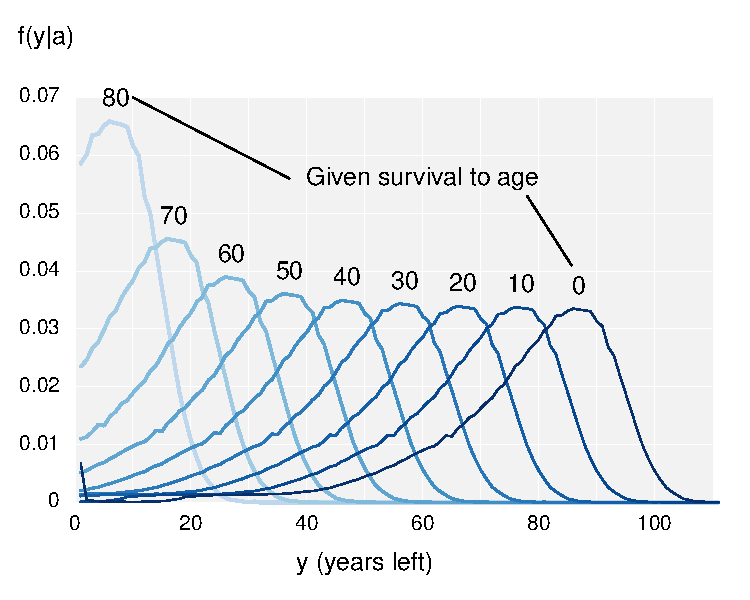
\includegraphics[scale=.8]{Figures/fya.pdf}	
	\caption*{*Note that $f(y|0) = d(a) = f(X)$.}
\end{figure}

$f(y|a)$ can be used to calculate the population having survived to age $a$ and
with $y$ remaining years of life as $P(a,y) = P(a)f(y|a)$, where the total
population with $y$ remaining years of life, $P(y)$, is simply $\int
_{a=0}^\infty P(a,y) \dd a$ \citep{brouard1986structure, brouard1989mouvements},
a single death cohort with members from many birth cohorts. This decomposition sorts the lifeline segments of a living population
by the part yet-unlived (years left) rather than by the part lived. 
The indices $a$ and $y$ differentiate between the past and future
parts of a lifeline, respectively, and by extension of populations when
so structured.
In comparing $P(a)$ with $P(y)$, as in \citet{brouard1986structure}, we still
refer to the living (lived or to-be-lived) part of a population.
Is it so clear that the dead are no longer part of the population? If a life is
completely saved, this life stays in the living population and is not counted
as a death, but we (in common thinking) often imagine saved lives as a transient
state classification.
Perhaps this is not correct for demographers: Among the living there
are no saved lives but only lived lives. Still we can quantify
hypothetically saveable life, and for this we must look to deaths.
It is nice, and often realistic, to think that many of the lives taken by death
are or will one day be saveable, but it is difficult to know what mortality
rates would apply to a population of saved individuals. Consider
the hypothetical population of lives saved a single time from death and subject to
the same mortality as the population at large.

Assume that all the deaths recorded in a year are saved and brought back to
life. One may ask much more than the number and age structure of these saved
lives, $D^s(a)$,
\begin{equation}
\label{eq:Dsa}
D^s(a) = \mu(a)P(a) \tc
\end{equation}
but also how many years the people saved at age $a$ would live, 
$W^s(a)$\footnote{A mnemonic for $W$ could be \textit{won} years. This is
essentially an age at death breakdown of YPLL.}? The simplest calculation is
to multiply the number of gained survivors by remaining life expectancy at each
age, $e(a)$:
\begin{align}
\label{eq:savedea}
W^s(a) = D^s(a)e(a) &= P(a)\mu(a)\frac{1}{l(a)}\int l(a+y) \dd y \tp
%\notag\\
         %&= \mu(a)\int_{y=0}^\infty B(t-a)l(a+y) \dd y 
\end{align}
$D^s(a)e(a)$ classifies potentially saved person-years by the
ages in which they were saved. One may also wish to know the distribution of remaining lifespans of saved
lives, which is quite different from \eqref{eq:savedea}:
\begin{equation}
\label{eq:savedya}
D^s(a)f(y|a) = P(a)\mu(a)\mu(a+y) \frac{l(a+y)}{l(a)} \tp
\end{equation}
Equation \eqref{eq:savedya} aggregates up to the thanatological age distribution
of saved lives, $D^s(y)$:
\begin{equation}
\label{eq:savedy}
D^s(y) = \int D^s(a)f(y|a) \dd a \tp
\end{equation}
%or the time-to-death distribution of the total years of life
%gained,
%\begin{equation}
%\label{eq:gainedy}
%W^s(y) = \int D^s(a)\frac{l(a+y)}{l(a)} \dd a \tc
%\end{equation}
Or one might ask through which chronological ages the gained years of life
would be lived, $W^s(a+y|a)$,
\begin{equation}
\label{eq:gaineday}
W^s(a+y|a) = D^s(a)\frac{l(a+y)}{l(a)} \tp
\end{equation}

Figure~\ref{fig:Day} (left) shows US 2010 period
deaths (all the lives that could be saved) by age and sex (males on the left,
females on the right). Over 1.23 million deaths were recorded for males
and females each in 2010 in the US. Deaths have been decomposed into discrete
categories of remaining years of life using equation~\eqref{eq:fya}, under the assumption that saved lives are subject to the same mortality schedule as the rest of the population, and under the supposition that all 2010 deaths get saved (just once). The results of this decompositon are represented by color bands in
Figure~\ref{fig:Day}. The average chronological age at death
for males was a full seven years lower than that for females
(69.9 versus, 76.9, respectively). Figure~\ref{fig:Dya} (right) displays the
same decomposition after swapping the y axis and color gradient from Figure~\ref{fig:Day}. Now thanatological age (years left) of hypothetically saved lives are the primary y axis, while chronological age groups (years lived) are displayed with color. Figure~\ref{fig:Dya} communicates that most saveable
lives would live short remaining lifespans once saved and granted the same lifetable
mortality. This is so in this data because most saveable lives are already in
chronological ages subject to high mortality rates. In general, the only
saveable lives that might live very long remaining lifespans are the few deaths that occur in young ages. 

Randomly
selected saveable males from this population would have on average longer
remaining lifespans than randomly selected saveable females (16.7 versus 13.3 years,
respectively). This is a paradox because females have lower mortality rates in
nearly all ages, and have longer remaining life expectancies in all ages. Female
mortality advantage is in this case more than offset by the relative youth of
male deaths. Untangling the paradox further becomes a recursive exercise,
since the relative youth of male deaths is due to an interaction between
mortality schedules and population structure, itself a result of past
vital forces.

\begin{figure}
\centering
\caption{US, 2010 potentially saveable lives (Deaths)}
\label{fig:1}
\begin{subfigure}[b]{.48\linewidth}
\centering
	\caption{Classified by age (years lived) and sex, and decomposed
by hypothetical remaining years of life (years left).}
	\label{fig:Day}
	% Figure produced in R/AllCauseFigures.R
	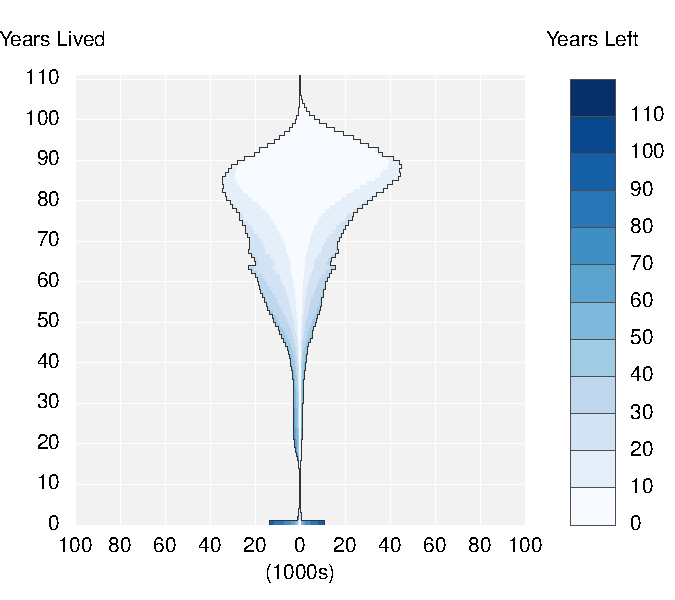
\includegraphics[scale=.55]{Figures/Deathsxy10.pdf}	
	\caption*{$D^s(a)$ from equation~\eqref{eq:Dsa}}
\end{subfigure}
~
\begin{subfigure}[b]{.48\linewidth}
\centering
    \caption{Classified by hypothetical remaining years of life
(years left) and sex, and decomposed by age (years lived).}
	\label{fig:Dya}
	% Figure produced in R/AllCauseFigures.R
    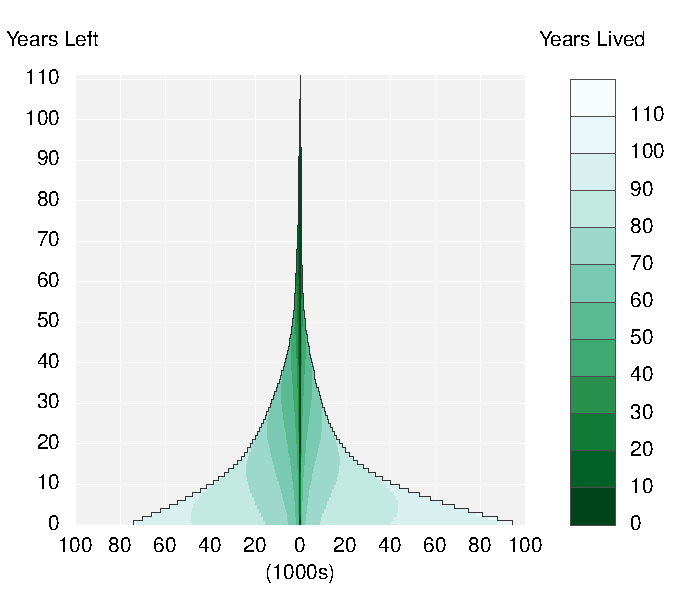
\includegraphics[scale=.55]{Figures/Deathsyx10.pdf}
    \caption*{$D^s(y)$ from equation~\eqref{eq:savedy}}
\end{subfigure}
\end{figure}

\begin{figure}
\centering
\caption{US, 2010 person years of life potentially won*}
\label{fig:2}
\begin{subfigure}[b]{.48\linewidth}
\centering
	\caption{Classified by age at hypothetical saving and sex, $W^s(a)$, and
	decomposed by future ages to be lived.}
	\label{fig:SavedGained}
	% Figure produced in R/AllCauseFigures.R
	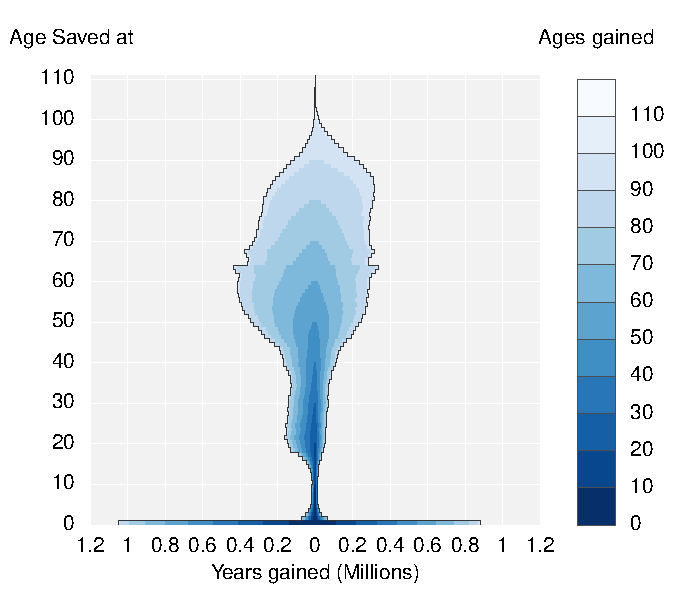
\includegraphics[scale=.55]{Figures/YearsSavedGainedxx10.pdf}
	\caption*{$W^s(a)$ from equation~\ref{eq:savedea}}	
\end{subfigure}
~
\begin{subfigure}[b]{.48\linewidth}
\centering
    \caption{Classified by cumulative ages to be lived through and sex, and
    decomposed by age at saving.}
	\label{fig:LostLived}
	% Figure produced in R/AllCauseFigures.R
    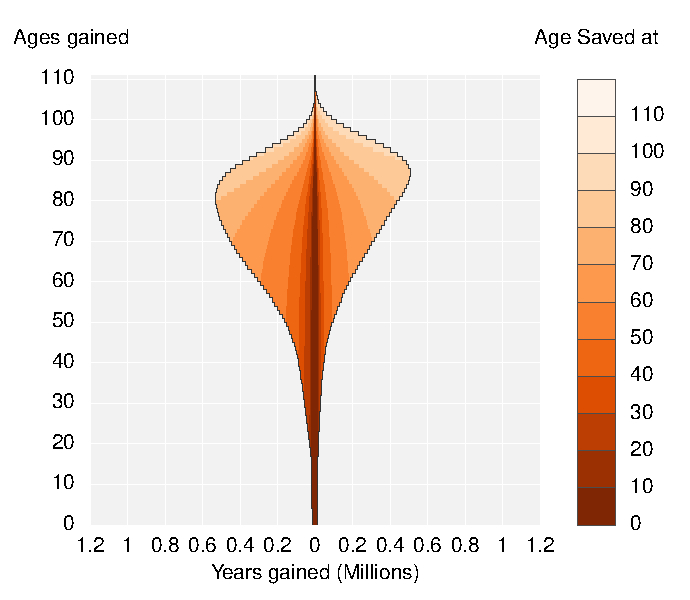
\includegraphics[scale=.55]{Figures/YearsLostLivedyx10.pdf}
    \caption*{$W^s(a+y|a)$ from equation~\ref{eq:gaineday}}	
\end{subfigure}
\caption*{*Note different x scale from Figure~\ref{fig:1}.}
\end{figure}

Figure~\ref{fig:SavedGained} shows the results of applying
equation~\eqref{eq:savedea} to the same US data, which is essentially a
reweighting of Figure~\ref{fig:Day} by remaining life expectancy. Color bands
are assigned by decomposing the total life to be lived into the ages through
which it will be lived. For example, if we save all 11700 of the 50-year-old US
males that died in 2010, they would live a total of 349000 combined years (under constant and
homogenous mortality), spread out over ages 50 and higher according to $\frac{l(50+y)}{l(50)}$. In Figure~\ref{fig:SavedGained} we decompose these
gained years of life according to equation~\eqref{eq:savedy} (using $f(a+y|a)$)
and highlight this decomposition with color, while in Figure~\ref{fig:LostLived}, \textit{gained} ages become the primary y axis,
and color bands represent the ages in which populations in each age group were
saved. 

Figure~\ref{fig:LostLived} represents the cumulative contribution to the
population pyramid that would result from saving all lives in 2010 and then
surviving them forward according to 2010 mortality conditions. The chronological
age axis indexes ages that are lived through at some point in the
future, in sequence rather than simultaneously. Under the same assumption of
fixed schedules, one could multiply this cumulative age structure with other
age-schedules, such as age-specific fertility rates, or the economic age profiles produced by
the NTA project, to benchmark the cumulative impacts of mortality on other
quantities of interest. For instance, the females
who died in 2010 would have given birth to 54122 babies cumulatively over their
remaining lifetime assuming they were subject to constant 2010 period fertility
\citepalias{HFD} and mortality. In the
following we work only with mortality data.

\section*{Causes of death}
% AS: Extension to causes of death. This is the case you want to make. Saying,
% for instance, what if we eliminate mortality from heart disease? Or stroke? or hypertension? We 
% need to explain an story here and the draft needs to be shaped according to
% that. I think that all your mathematical material is very relevant but we need to get deeper into 
% the general idea and maybe leave the formulas for an appendix. But it is ok
% for the moment, we will think about that later.

These basic relationships carry over when deaths and survival are adjusted to
account for the hypothetical elimination of particular causes (in the case of
independence). In this case $D^s$ is the sum of $n$ causes, and to speak of
eliminating cause $c$ from the lifetable is to speak of saving $D^{sc}$ lives and then
subject them to the mortality conditions of all causes except $c$.
This is problematic in that causes are not independent, and also in that
reductions in cause-specific mortality are not so thorough and immediate, but it
serves as a good basis for comparing the relative impacts of different causes on
a given population structure. Humans have succeeded in eradicating certain
causes of death in the past, and it
is not so audacious to imagine that we may do so yet. While these
eliminations may not deduct 100\% of their magnitude from all-cause mortality
due to substitution, there is an undeniable all-cause benefit, and at least 
we know its bounds. For some causes of death, independence is easier to imagine,
such as deaths due to needless violence or particular kinds of accidents. We
demonstrate concepts using large cause groupings.

Define the force of mortality, $\mu(a) = \sum _{c=1}^n \mu^c(a)$,
as the sum of $n$ categorically separable causes. The people that will die from
cause $c$ are:
\begin{align}
D^c &= \int_0^\infty D^c(a) \dd a \\
&= \int_0^\infty \mu^c(a)P(a) \dd a \tc\\
\intertext{and to hypothetically save all these people is to remove cause $c$
from mortality, retaining $D^c$ lives in the population. It makes sense to
calculate the distribution of remaining lifespans of the $D^c$ people that would
have died of this cause using $l(a)$ removed of the cause in question, so we define
$l^{-c}(a)$,}
l^{-c}(a) &= e^{-\int _0^a \mu(a)-\mu^c(a) \dd a} \tc\\
\intertext{which is hopefully more legible to render as}
l^{-c}(a) &= e^{-\int _0^a \mu^{-c}(a) \dd a} \tp\\
\intertext{This is a stronger supposition than the idea of repeated
resuscitation from \citet{vaupel1987repeated}, but the idea is to separate out
the impacts of particular causes.
Let us continue with the same notational concept of ${ }^{-c}$ to define
remaining life expectancy assuming survival to age $a$ and no more death from cause $c$ after age $a$, $e^{-c}(a)$:} e^{-c}(a) &= \frac{1}{l^{-c}(a)}\int _{y=0}^\infty l^{-c}(a+y) \dd y \tp
\end{align}
and so on, repeating equations \eqref{eq:savedea} and \eqref{eq:savedy} for the
case of cause-specific saveable lives and their cause-deleted remaining
lifespans.

Now Figures~\ref{fig:1} and~\ref{fig:2} can be repeated for
any particular cause of death, and the profile of each of the four perspectives
characterizes the population impact of the given cause of death.
Figures~\ref{fig:3} and~ \ref{fig:4} depict the same temporal viewpoints,
respectively, but now the deaths decomposed are only deaths to external
causes, and external causes have been eliminated from the lifetable functions used for decomposition and
 redistribution. Causes differ in their impact profiles, and this forms a
 basis for comparison. As with standard population pyramids, one may prefer the
 use of percent scales to facilitate comparisons between causes or countries. These
 figures for external causes give visual form to the intuition that demographers
 aleady have about external causes of death. External causes are important in
 young ages, and affect males more than females. Saving a randomly selected death from an external
 cause will on average have a higher payoff in terms of expected years of life gained than does preventing a death in general. Further,
 a typical life saved will traverse many working ages, and reach well into old
 ages.
 The group with the most to gain by eliminating external causes are males in
 their 20s (clearest in Figure~\ref{fig:4}).
 
 The average chronological age of deaths to external causes in the USA in 2010
 was 47.9 for males and 57.1 for females. Their cause-deleted mean remaining
 lifetimes were 34.0 and 29.8 years, respectively. The mean age-at-saving of all
 the person-years hypothetically won under these same conditions becomes 36.7
 for males and 40.3 for females, whereas the mean of the ages \textit{enjoyed}
 by these hypothetically saved people are 59.7 and 63.3, respectively. Means do
 not tell the story as well as images. 

\begin{figure}
\centering
\caption{USA, 2010 Deaths from external causes}
\label{fig:3}
\begin{subfigure}[b]{.48\linewidth}
\centering
	\caption{Classified by age (years lived) and sex, and decomposed
by hypothetical remaining years of life (years left).}
	\label{fig:Dayc}
	% Figure produced in R/SingleCauseExampleFigures.R
	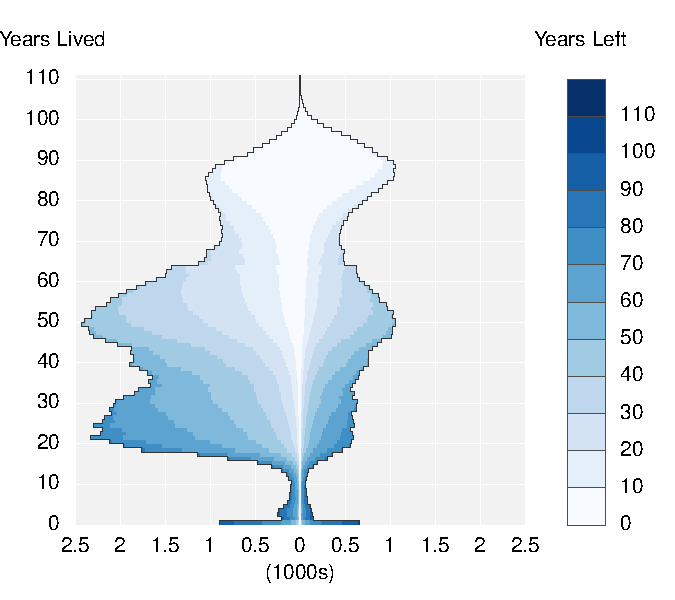
\includegraphics[scale=.55]{Figures/Deathsxy10USAExternal.pdf}	
	\caption*{$D^{sc}(a)$}
\end{subfigure}
~
\begin{subfigure}[b]{.48\linewidth}
\centering
    \caption{Classified by hypothetical remaining years of life
(years left) and sex, and decomposed by age (years lived).}
	\label{fig:Dyac}
	% Figure produced in R/SingleCauseExampleFigures.R
    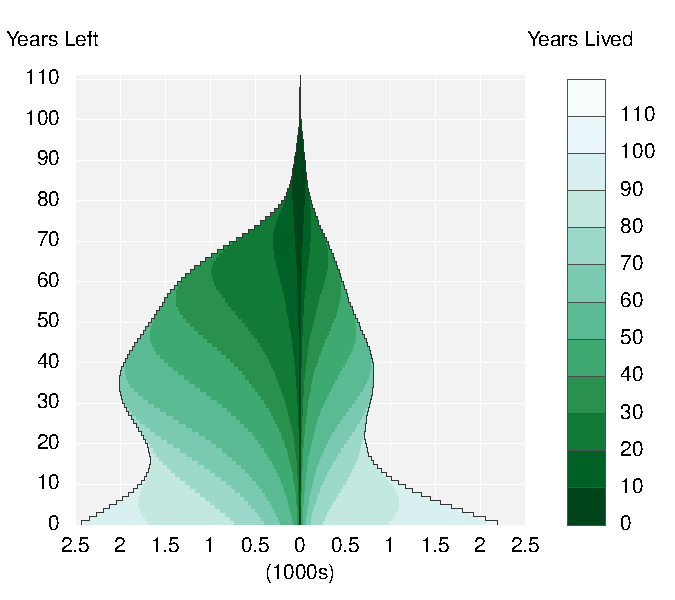
\includegraphics[scale=.55]{Figures/Deathsyx10USAExternal.pdf}
    \caption*{$D^{sc}(y)$ }
\end{subfigure}
\end{figure}


\begin{figure}
\centering
\caption{USA, 2010 Deaths from external causes, years of life potentially won*}
\label{fig:4}
\begin{subfigure}[b]{.48\linewidth}
\centering
	\caption{Classified by age at hypothetical saving and sex, $W^s(a)$, and
	decomposed by future ages to be lived.}
	\label{fig:SavedGainedUSAExternal}
	% Figure produced in R/SingleCauseExampleFigures.R
	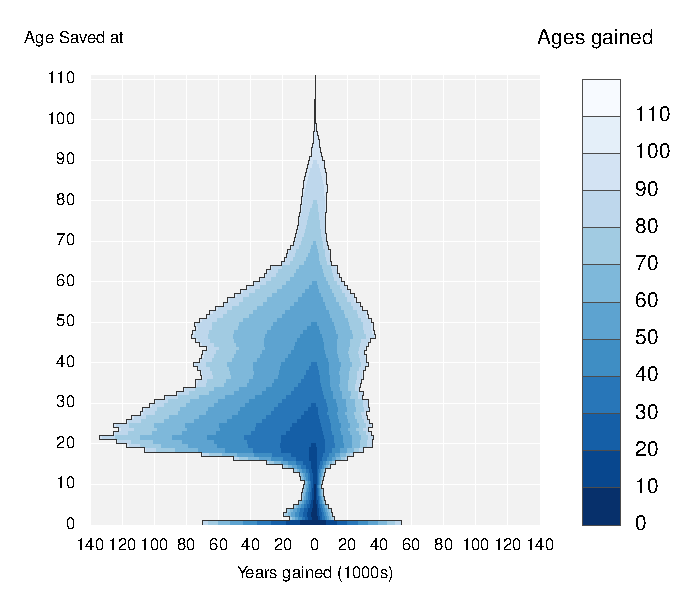
\includegraphics[scale=.55]{Figures/YearsSavedGainedxx10USAExternal.pdf}
	\caption*{$W^s(a)$ from equation~\ref{eq:savedea}}	
\end{subfigure}
~
\begin{subfigure}[b]{.48\linewidth}
\centering
    \caption{Classified by cumulative ages to be lived through and sex, and
    decomposed by age at saving.}
	\label{fig:LostLivedUSAExternal}
	% Figure produced in R/SingleCauseExampleFigures.R
    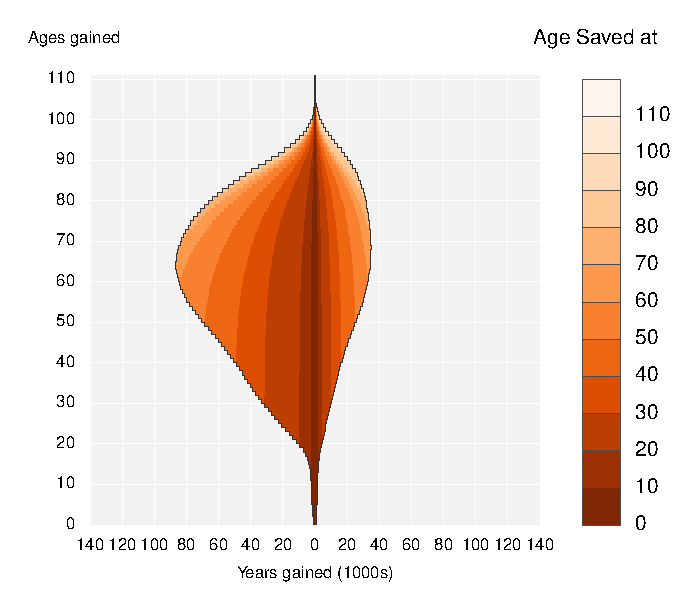
\includegraphics[scale=.55]{Figures/YearsLostLivedyx10USAExternal.pdf}
    \caption*{$W^s(a+y|a)$ from equation~\ref{eq:gaineday}}	
\end{subfigure}
\caption*{*Note different x scale from Figure~\ref{fig:3}.}
\end{figure}

\FloatBarrier

\section*{Observed patterns}
In this section we summarize cause of death impacts from eight
major cause groups: cancers, cardiovascular disease, external causes, ill-defined casues, infant and congenital causes, infectious disease, mental
debilitation, and other causes. These results will be summarized for the USA,
Canada, England and Wales, Norway, and Sweden based on a soon-to-be
released collection from the HMD. This section may have a supplemental appendix
of results.

\section*{Discussion}

There are many perspectives under which the demography can account for the
relationships between stocks and flows, but not all form part of the collective
practice of demography. 
Our objective in these exercises has been to offer a novel quantitative and
visual basis to assess the impact of mortality on population stocks.
This is done by calculating the lifespan distributions foregone due to death and indexing the results based on various aspects of the lifespan. Practical suggestions have included both chronological and thanatological age
perspectives, as well as two ways of accounting for years of lifespan gained:
(i) The years would be won by saving the deaths in age $a$, and (ii) the
ages saved individuals would pass through if survived forward.

The reader may choose to interpret this exercise as we
have narrated it: ``what would have happened if these lives had been saved?''. We wish to point out that believing
this statement is not necessary in order for the measures to be useful, just as common uses of
period life expectancy require a certain degree of suspended disbelief. For
clarity, we list the most important assumptions to be aware of when treating
data as we have.
\begin{enumerate}
\item Unchanging period rate schedules. Note that the same formulas apply when
data in the cohort perspective are used, but some care must be taken to allocate past deaths according to observed mortality within the cohort, and then complete non-extinct
cohorts' mortality experience according to
projection. \citet{brouard1986structure} combined history and projection
in this way in his original study of population structure.  In any case, period measures are the best barometer of the
present that we have, and all calculations done in this paper fall under the
period umbrella. The researcher is not limited to the use of static age
schedules, and $f(y|a)$ could be calculated for age schedules that vary
by birth cohort.
\item Homogenous populations. In using rate schedules derived from the
population at large in order to describe a hypothetical population of saved
individuals, we may neglect that saved individuals may be a frailer than the
general population, and so subject to higher mortality rates going forward. We
offer to remedy for this shortcoming, except to note that this possibility may
hold truer for some causes than for others, and in general the degree of bias is
unknown.
\item Independence of causes. As discussed in the text, all causes of death
compete to be first, and removing the first cause may not reduce the all cause
rate by the same amount we have partitioned, $\mu^c$. The final reduction will
lie somewhere between 0 and $\mu^c$, and may depend on the cause and
overall level of mortality. We think that this possible unsolvable limitation
ought not keep the researcher from exploring in this direction.
\end{enumerate}



%Then, decide whether to present a separate panel for each country of all causes
%for each perspective, or rather each cause in a unique panel comparing
%countries. I'm leaning toward each each country in a separate panel, but need
% to think on it more. I'm doubting whether it makes sense to compare populations
%that are not stable, since part of differences will be due to previous
%population structure. Comparing causes (save for competing risks) works within
% a population because it has a single structure, but between countries it may only
%make sense to go back to rates, but then we lose the point of the paper. This
% is my tentative stance on between-country comparisons. It's of course all easy to
%decompose, but that seems like a frivolous step.
% AS: Regarding expanding the analysis to more populations, I think that you are
% right, but part of the differences would be not only due to the structure but the context 
% of each population.
% 
---------------------------------------
\bibliographystyle{plainnat}
  \bibliography{references}  
\end{document}
